\subsection{Descripción del problema.}

\vspace*{0.3cm}

Este problema se trata de implementar un algoritmo que, de ser posible,
\textbf{calcule la cantidad mínima de saltos} que debe dar un participante para poder cruzar un
puente de cierto tamaño (fijo), el cual presenta \textbf{algunos de sus tablones rotos}. Estos se encuentran
marcados y \textbf{deben ser evitados}, de otro modo, el participante fracasa en su intento y puede llegar a
perder la vida. Cada uno de los participantes puede saltar una \textbf{determinada cantidad de tablones como máximo}. \medskip

El algoritmo debe decidir si dicha hazaña es posible, y de ser así,
\textbf{especificar la cantidad de saltos a dar y a qué tablones hacerlo}. \medskip

Asumimos que tanto la \textbf{longitud del puente como la cantidad de saltos máximos por participante
son valores naturales}.

\vspace*{0.5cm}

\textbf{Ejemplos:}
\begin{itemize}
  \item Para un puente de 10 tablones y un participante capaz de saltar de a 3
  tablones como máximo, teniendo los tablones 1, 4, 6, 8 y 9 rotos, la salida podría ser:
  primero saltar al tablón 3, luego al 5, luego al 7, luego al 10 y luego fuera del puente.
  \item Si en cambio, en el ejemplo anterior, el tablón 7 también estuviese roto,
  el algoritmo debe informarnos que, bajo esas condiciones, no es posible cruzar el puente.
  \item \textcolor{red}{\textbf{agregar un ejemplo mas con dibujitos y cosas lindas!}}
\end{itemize}



\subsection{Desarrollo de la idea y pseudocódigo.}

\vspace*{0.3cm}

Para resolver este problema, propusimos un algoritmo de tipo \textit{greedy}, que en cada iteración
del mismo busca siempre saltar \textbf{la mayor cantidad posible de tablones}, siempre y cuando el
tablón al que nos dirijamos esté sano. Caso contrario, se saltará al tablón anterior (ó al anterior), 
y así sucesivamente, hasta encontrar un tablón válido.
Si retrocediendo de este modo se llega a la posición en la que se encuentran el competidor, el problema
\textbf{no tiene solución}.

\vspace*{0.5cm}


\begin{codebox}
\Procname{$\proc{cruzarPuente}(n,c,puente)$}
\li \Comment n: cantidad de tablones del puente puente es el vector
\li \Comment c: cantidad de tablones máximos a saltar
\li \Comment puente: es el conjunto de tablones
\li \Comment el primer tablón es el 1
\li $\id{solucion} \gets \emptyset$
\li \If $\id{c} > \id{n}$
\li     \Then
            $\proc{agregar}(solucion, c)$
\li         \Return $\id{solucion}$
        \End
\li \If $\neg(\proc{esPosibleCruzar}(puente, c))$
\li     \Then
            \Return $\emptyset$
        \End
\li $\id{posicionActual} \gets 0$
\li \While $\id{posicionActual} \leq \id{n}$
\li     \Do
            $saltoActual \gets c$
\li         \While $\neg(\proc{puedeSaltar}(puente, posicionActual + saltoActual - 1))$
\li         \Do
                $saltoActual \gets saltoActual - 1$
            \End
\li     $\id{posicionActual} \gets \id{posicionActual} + \id{saltoActual}$
\li     $\proc{agregar}(solucion, posicionActual)$
        \End
\li \Return $\id{solucion}$
\end{codebox}


\vspace*{0.5cm}


\begin{codebox}
\Procname{$\proc{puedeSaltar}(puente, tablon)$}
    \Return $\id{tablon} \geq \proc{tamanio}(puente) \lor \proc{estaSano}(puente[tablon])$
\end{codebox}


\vspace*{0.5cm}


\begin{codebox}
\Procname{$\proc{esPosibleCruzar}(puente, c)$}
\li \Comment c: cantidad de tablones máximos a saltar
\li $\id{tablonesRotosConsecutivos} \gets 0$
\li \For $i \gets 0$ \To $\proc{tamanio}(puente) - 1$
\li     \Do
            \If $\proc{puedeSaltar}(puente, i)$
\li             \Then
                    $\id{tablonesRotosConsecutivos} \gets 0$
\li         \Else
\li             $\id{tablonesRotosConsecutivos} \gets \id{tablonesRotosConsecutivos} + 1$
            \End
\li         \If $\id{tablonesRotosConsecutivos} \geq c$
\li             \Then
                    \Return $\const{false}$
            \End
        \End
\li \Return $\const{true}$
\end{codebox}



\subsection{Justificación de la resolución y demostración de correctitud.}

\vspace*{0.3cm}

Antes de comenzar, diremos que una solución $S$ es de la forma $s \ t_1 \dots t_s$,
siendo $s$ la cantidad de saltos y $t_i$ el $i$-ésimo tablón al cual saltar. $S$ se considera
\textit{óptima} si $s$ es \textbf{mínimo}. También definiremos la relación entre soluciones $\sqsubseteq$, que,
dadas $S = s \ t_1 \dots t_s$ y $H = h \ u_1 \dots u_h$, se da del siguiente modo:
\begin{align*}
  S \sqsubseteq H \iff s \leq h \wedge \bigwedge_{i=1}^s t_i = u_i
\end{align*}

Para demostrar que el algoritmo propuesto es correcto para la resolución de este problema,
separaremos las entradas en casos y analizaremos éstos a continuación.

\begin{itemize}
  \item $c > n$: en este caso, la solución será de la forma $1 \ k$, con $k > n$. Como $c > n$, la
  solución $1 \ c$ es una solución posible (y óptima).

  \item $c \leq n$: si la instancia no tiene solución, es porque hay $c$ o más tablones
  consecutivos rotos. En tal caso, la función \textsc{esPosibleCruzar} se encarga de
  decirnos si hay solución. Más adelante demostraremos que \textsc{esPosibleCruzar}
  también es correcta. \medskip

  En cambio, si tiene solución, plantearemos el siguiente esquema:

  \begin{codebox}
  \Procname{$\proc{Greedy}(S,f,p)$}
  \li \Comment $S$ es el conjunto de tablones
  \li \Comment $f$ es una función que elige el tablón mas lejano que se puede saltar
  \li \Comment $p(A, x)$ es una función que indica si a una subsolución $A$ se le
  \li \Comment   puede agregar el tablón $x$. Es decir, si está sano y a una distancia
  \li \Comment   a lo sumo igual al salto máximo del último tablón agregado.
  \li $\id{S^{opt}} \gets \emptyset$
  \li \While $\id{S} \neq \emptyset$
  \li     \Do
    			$\id{x} \gets f(S)$
  \li  			$\id{S} \gets \id{S} \setminus \{\id{x}\}$
  \li			\If $p(S^{opt}, x)$
    				\Then
  \li					$\id{S} \gets \id{S} \setminus \{\id{c} \mid \id{c} < \id{x}\}$
  \li					$\id{S^{opt}} \gets \id{S^{opt}} \cup \{\id{x}\}$
    				\End
    		\End
  \li \Return $\id{S^{opt}}$
  \end{codebox}

  \textbf{Demostración (\textsc{cruzarPuente}):}
  \begin{itemize}
    \item Definimos como \textbf{subsolución} a un conjunto de tablones, que
    es \textbf{subconjunto de una solución óptima}.
    \item $S^{opt}$ empieza siendo $\emptyset$, que es subconjunto de cualquier
    solución óptima (si tal solución existe). Inicialmente se calcula si
    existe forma de cruzar el puente, por lo que al llegar a este punto del
    algoritmo, se puede estar seguro que existe una solución.
    \item Supongamos que estamos en la iteración k-ésima. Al iniciar
    el ciclo, $S^{opt}$ es una subsolución de la solución óptima $S^{*}$. \medskip
    
    Sea $S^{opt} \sqsubseteq S^{*}$ y $\id{x} \gets F(S)$. \medskip
    
    En esta iteración, podemos: \medskip
    
    $(a)$ No agregar $x$ a $S^{opt}$
    
    $(b)$ Agregar $x$ a $S^{opt}$ \medskip
    
    Si sucede $(a)$, entonces no se modifica $S^{opt}$, por lo tanto sigue
    siendo \textbf{subsolución de $S^{*}$}, es decir, es una \textbf{solución óptima}. \medskip
    
    Si sucede $(b)$, agregamos $x$ (aplicamos $f(S)$), es decir, el tablón más
    lejano al cuál se puede saltar. Como lo estamos agregando, vale
    $p(S^{opt}, x)$, es decir, que $x$ es un tablón sano. \medskip
    
    Sea $S'^{opt} \gets S^{opt} \cup \{x\}$. Queremos ver que existe una
    solución óptima $S'^{*}$, tal que $S'^{opt} \sqsubseteq S'^{*}$. \medskip
    
    Tenemos, nuevamente, dos casos: \medskip 
    
    $(a')$ $x \in S^{*}$
    
    $(b')$ $x \notin S^{*}$ \medskip
    
    Si sucede $(a')$, entonces $S'^{opt} \sqsubseteq S^{*}$. 
    Tomamos $S'^{*} \gets S^{*}$, una solución óptima. \medskip 
    
    Caso $(b')$. Sean $x'$ el \textbf{mínimo valor} de $S^{*} \setminus S^{opt}$, 
    $u$ el máximo valor de $S^{opt}$ (es decir, la última posición a la que
    se saltó) y $u'$ el mínimo valor de $S^{*} \setminus (S^{opt} \setminus \{x'\})$, es
    decir, el valor siguiente a $x'$ en $S^{*}$.
    
    Como $x \notin S^{*}$, $x$ no puede ser igual a $x'$. Entonces $x' > x$.
    Pero el salto de $u$ hacia $x'$ es válido, porque $S^{*}$ es una solución
    válida. Es \textbf{absurdo}, porque definimos $f$ como la función que nos
    da la mayor posición válida y en este caso retornó $x$ en lugar de $x'$.
    
    Por lo tanto, sólo puede valer $x > x'$. En este caso, consideremos a
    $S'^{*} \gets S^{*} \setminus (\{x'\} \cup \{x\})$. El salto de $u$ hacia $x$ es
    válido, porque así lo indica $p(S^{opt}, x)$ y el salto de $x$ hacia $u'$
    es menor que el de $x'$ hacia $u'$. Por lo tanto, si el salto de $x'$ es válido,
    el de $x$ también. La cantidad de saltos de $S'^{*}$ es exactamente igual a la de 
    $S^{*}$, ya que consiste simplemente en reemplazar un elemento por otro.
    
    Entonces $S^{opt} \sqsubseteq S'^{*}$, es una \textbf{subsolución de una solución óptima}.
    
    \item Al terminar el ciclo, recorremos todos los tablones y vemos que $S^{opt}$ 
    es subsolución de una solución óptima. Sea $S^{*}$ tal solución óptima.
    Si $S \gets S^{*}$ entonces $S^{opt}$ es una solución óptima.
    
    Si no, $\exists x \in (S^{*} \setminus S^{opt})$. Pero $x \in S$ y $p(S^{*}, x) \gets \const{true}$,
    por lo tanto $p(S^{opt}, x) \gets \const{true}$ y $P(X, x) \gets \const{true}$, para todo prefijo
    X de $S^{opt}$. Entonces, al momento de sacar $x$ de $S$ e intentar agregarlo a $S^{opt}$, 
    deberíamos poder, pero no es lo que sucede. 
    
    Esto no puede pasar, luego no existe $x$, y $S^{*} \gets S^{opt}$.

  \end{itemize}

\newpage

\textbf{Demostración (\textsc{esPosibleCruzar}):} 
\begin{itemize}
\item La función \textsc{esPosibleCruzar} mantiene un \textbf{contador de tablones rotos consecutivos},
inicializado en 0. Recorre todos los tablones \textbf{en orden}; si el tablón actual
está sano, resetea el contador a 0, sino (está roto) le suma 1.
Luego, si en algún momento el contador es \textbf{mayor ó igual al salto máximo posible},
devuelve \textbf{falso}. En cambio, si se recorren todos los tablones y esto no sucede, 
la función devuelve \textbf{verdadero}.

Por lo tanto, la función devuelve falso $\iff$ existe en algún momento una
cantidad de tablones rotos consecutivos mayor o igual al salto máximo. 

Veamos que esto es equivalente a que el puente pueda ser cruzado: \medskip

\textbf{Teorema:} Es posible cruzar un puente $\iff$ su cantidad de tablones rotos
consecutivos es menor al salto máximo. \medskip

\item \textbf{Demostremos la ida:}
Sea un puente de $n$ tablones, con un salto máximo de $c$ y una cantidad máxima de
tablones rotos consecutivos $k$.
Supongamos $k \geq c$.
Si es posible cruzarlo, entonces existe una solución $S$, que consiste en una
secuencia de saltos.
Sean $t_1$ el primero de los tablones y $t_c$ el tablón correspondiente a la posición $c$, entre 
los tablones consecutivos rotos (que sabemos que existe porque c $\leq$ k).
Sea $s_0 \in S$ la posición (en tierra o en un tablón) máxima anterior a $t_1$ y sea $s_1 \in S$ 
la posición inmediata siguiente a $s_0$.
Dado que $c$ es el salto máximo, entonces $s_1 - s_0 \leq c$ ó, lo que es lo
mismo, $s_0 + c \geq s_1$.
Elegimos $s_0 < t_0$, entonces $s_0 + c < t_0 + c$.
Pero esto es $s_0 + c < t_c$ y $s_1 \leq s_0 + c < t_c$.

Entonces, o bien $s_1 < t_0$ (que resulta imposible, pues se eligió $s_0$ como el máximo
menor a $t_0$), ó $t_0 \leq s_1 < t_c$, pero entonces el salto se hubiera realizado a un
tablón roto. \medskip

\textbf{¡Absurdo!}, que viene de suponer que existe una solución cuando la cantidad de
tablones rotos consecutivos es igual o mayor al salto máximo. \medskip

\item \textbf{Demostremos la vuelta:}
Sea un puente de $n$ tablones, con salto máximo $c$ y cantidad máxima de
tablones rotos consecutivos $k$, con $k < c$.
Sea $S$ la solución que consiste en caer en todos los tablones sanos y luego al
otro lado del puente (es decir, cruzarlo).

Esta solución cruza el puente completamente y para cada posición 
$s_i \in S, 1 \leq s_{i+1} - s_i \leq k$, ya que no saltea tablones sanos.
Entonces $s_{i+1} - s_i \leq k => s_{i+1} - s_i \leq c$. 

Por lo tanto todos los saltos en $S$ son válidos y la solución existe.
\end{itemize}

\end{itemize}



\subsection{Análisis de complejidad.}

\vspace*{0.3cm}

Para el análisis de complejidad nos basaremos en el pseudocódigo de la función 
\textsc{cruzarPuente}, correspondiente al ítem \textbf{3.2}.

\begin{enumerate}
  \item Todas las operaciones realizadas sobre el contenedor \verb|vector| de la \textit{STL} (size, push_back, empty y la creación de iteradores)
  toman tiempo constante $O(1)$.

  \item Las asignaciones realizadas (11, 13, 15, 16 y 17) también se realizan en tiempo constante $O(1)$.

  \item Si $c$ es mayor que $n$ (línea 6), retornamos el vector de soluciones que contiene la cantidad de saltos realizados (cero) y
  el "tablón" $c$ hacia el cual saltamos. Como dijimos anteriormente, realizar estas operaciones sobre \verb|vector|
  toma tiempo constante $O(1)$.

  \item En la línea 9, ejecutamos el condicional \verb|esPosibleCruzar(puente, c)|. La complejidad de esta función la
  analizaremos luego, pero adelantamos que es lineal, $O(n)$.

  \item En la línea 12 (tener en cuenta que en este caso vale $c \leq n$), en el peor caso ($c = 1$), realizamos $n$ iteraciones,
  pues recorremos el puente de a un tablón (siempre y cuando no haya tablones rotos, pues no tendría solución). Con $c \neq n$,
  en cualquier iteración podemos realizar a lo sumo $c$ retrocesos, pero en las siguientes esto es compensado, pues sabiendo que
  hay solución, la metodología empleada no pregunta más de 1 vez el estado de un mismo tablón. Este procedimiento tiene como peores
  casos los siguientes:
  \begin{itemize}
    \item $c = 1$, con todos los tablones sanos, de manera que haya que chequear todos los tablones del puente.

    \item $c = 2$, con un patrón de tablones sano - roto - sano, como se puede ver en la figura \textcolor{red}{\textbf{QUE DESPUES AGREGAMOS!}}

    \item $c = n$, con todos los tablones rotos salvo el primero, de manera que haya que chequear todos los tablones del puente.
  \end{itemize}

  \item La complejidad de \verb|esPosibleCruzar(puente, c)| (línea 9) es $O(n)$, pues en el peor caso recorre el puente entero.

  \item La complejidad de \verb|puedeSaltar(puente, tablón)| es $O(1)$, pues obtenemos el tamaño del puente en tiempo constante
  mediante la función \verb|size| y preguntar si un tablón está sano ó no es constante.

\end{enumerate}

Por lo tanto, la \textbf{complejidad total} del algoritmo implementado para este problema es

\begin{align*}
  O(1) + O(1) + O(n) + O(n)*O(1) = \textit{\textbf{O(n)}}
\end{align*}



\subsection{Experimentación y gráficos.}

\vspace*{0.3cm}

\subsubsection{Test 1 - benchmark caso aleatorio}

En este test, fijamos el valor de $c$ (salto máximo) en 20, mientras que $n$ (cantidad de tablones) 
se inicializa en 1000 y va incrementándose también de a 1000, hasta alcanzar 1000000. La 
distribución de los tablones rotos/sanos se genera aleatoriamente, de forma uniforme.
 
Para cada instancia, se toma el \textbf{valor mínimo} de cantidad de ciclos luego de \textbf{25 corridas}. 

\vspace*{0.5cm}

\begin{figure}[h]
  \begin{center}
    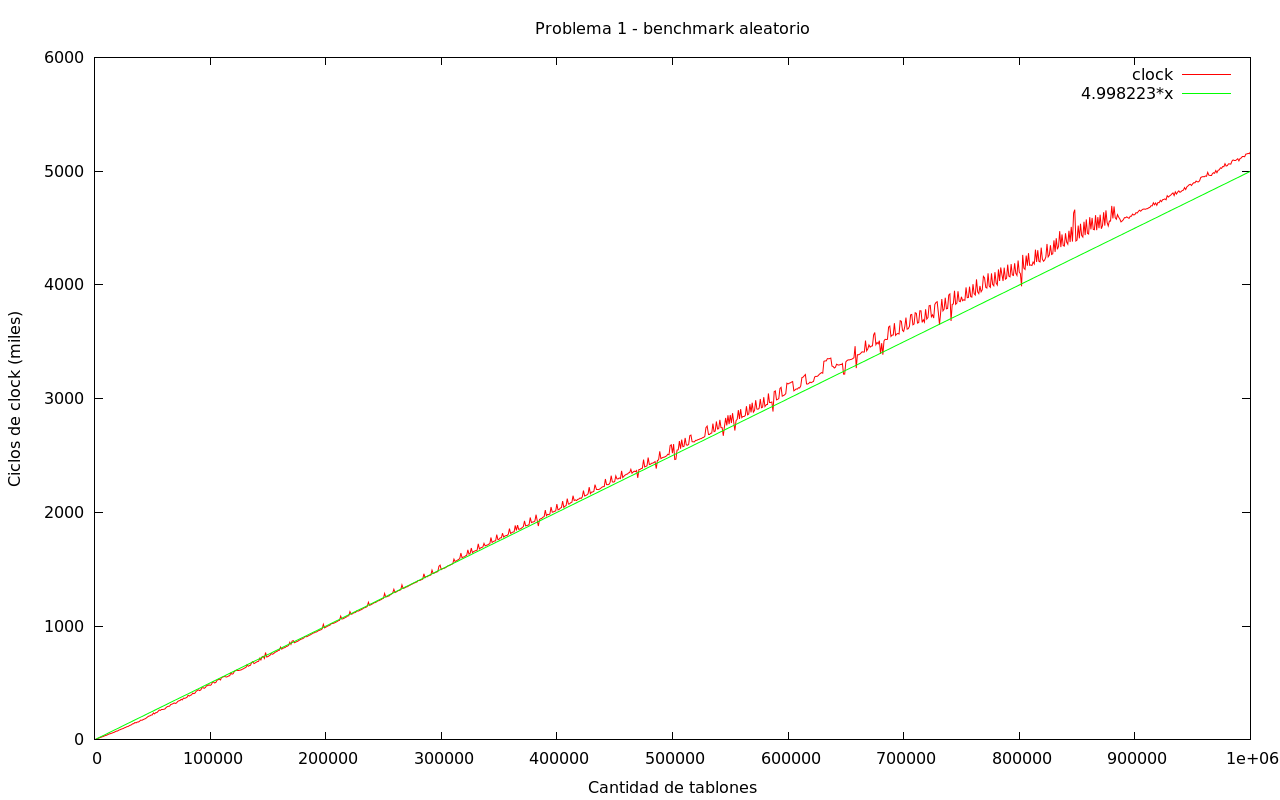
\includegraphics[scale=0.35]{imagenes/grafico-1.png}
  \end{center}
\end{figure}

\vspace*{0.5cm}

En este gráfico podemos apreciar que, a partir de cierto valor $n_0$ (aproximadamente 300000), la 
curva se comporta como una recta, es decir, \textbf{tiene complejidad lineal}, tal como habíamos 
advertido en el análisis teórico de complejidad realizado anteriormente. También puede observarse, en 
el inicio, que la cantidad de ciclos requeridos para ejecutar el algoritmo crece mucho en comparación 
a los valores posteriores. Esto puede explicarse por que el procesador debe realizar ciertos cálculos que 
luego, al notar cierto patrón sobre las instancias y operaciones realizadas, no vuelve a computar, 
reduciendo así la cantidad de ciclos requeridos.


\newpage


\subsubsection{Test 2 - benchmark del peor caso}

En este test, fijamos el valor de $c$ (salto máximo) en 1, mientras que $n$ (cantidad de tablones) 
se inicializa en 1000 y va incrementándose también de a 1000, hasta alcanzar 1000000. Todos los 
tablones se encuentran sanos.

Para cada instancia, se toma el \textbf{valor mínimo} de cantidad de ciclos luego de \textbf{25 corridas}.

\vspace*{0.5cm}

\begin{figure}[h]
  \begin{center}
    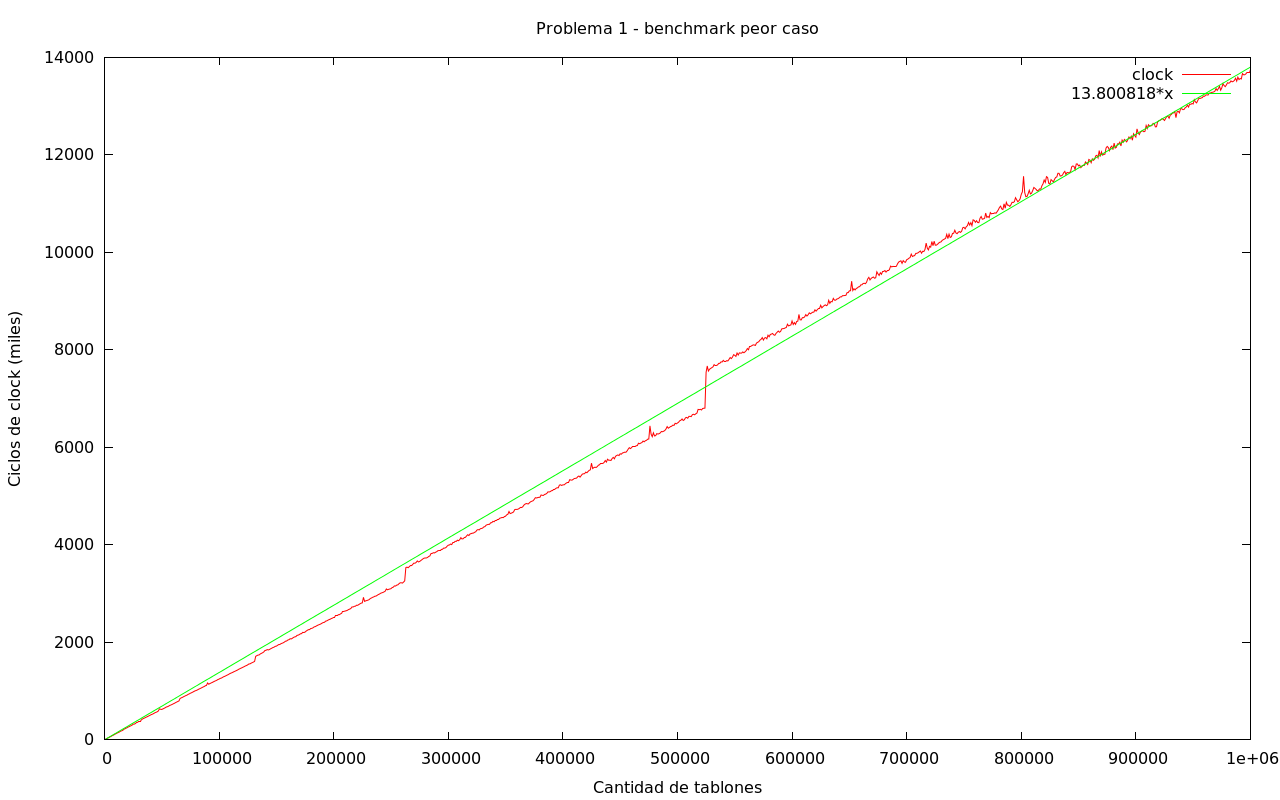
\includegraphics[scale=0.35]{imagenes/grafico-1-peor.png}
  \end{center}
\end{figure}

\vspace*{0.5cm}

En este gráfico podemos apreciar que, a diferencia del caso anterior, \textbf{el algoritmo debe realizar todas
las comparaciones (no saltea tablones)}, por lo cual el tiempo consumido por el mismo aumenta significativamente. 
Si bien los gráficos muestran un comportamiento similar, \textbf{la diferencia clave es la cantidad de ciclos 
necesarios para ejecutar esta instancia}.


\newpage


\subsubsection{Test 3 - benchmark del mejor caso}

En este test, fijamos el valor de $c$ (salto máximo) en X, mientras que $n$ (cantidad de tablones) 
se inicializa en X y va incrementándose también de a X, hasta alcanzar 1000000. Todos los 
tablones se encuentran sanos.

Para cada instancia, se toma el \textbf{valor mínimo} de cantidad de ciclos luego de \textbf{25 corridas}.


\begin{figure}[h]
  \begin{center}
    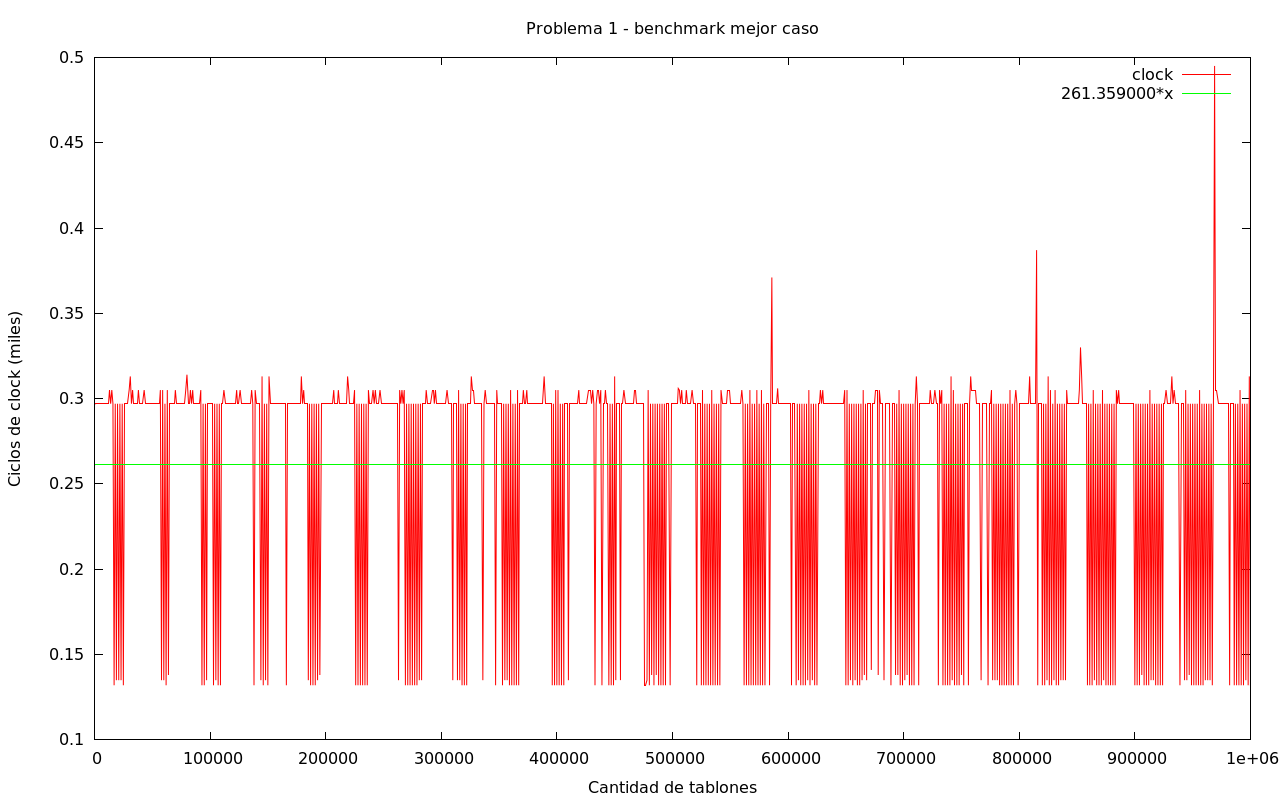
\includegraphics[scale=0.35]{imagenes/grafico-1-mejor.png}
  \end{center}
\end{figure}


En este gráfico podemos apreciar que, a pesar de algunas \textit{perturbaciones} esporádicas, la complejidad 
se mantiene constante, a diferencia del caso aleatorio y peor, donde la misma era lineal. Además, la cantidad de 
ciclos se ve muy reducida en comparación a la cantidad requerida para valores similares de $n$ en los casos anteriores.


\newpage


\subsubsection{Test 4 - benchmark con saltos aleatorios}

En este test, fijamos el valor de $n$ (cantidad de tablones) en 100000, mientras que el valor 
.

Para cada instancia, se toma el \textbf{valor mínimo} de cantidad de ciclos luego de \textbf{25 corridas}.


\begin{figure}[h]
  \begin{center}
    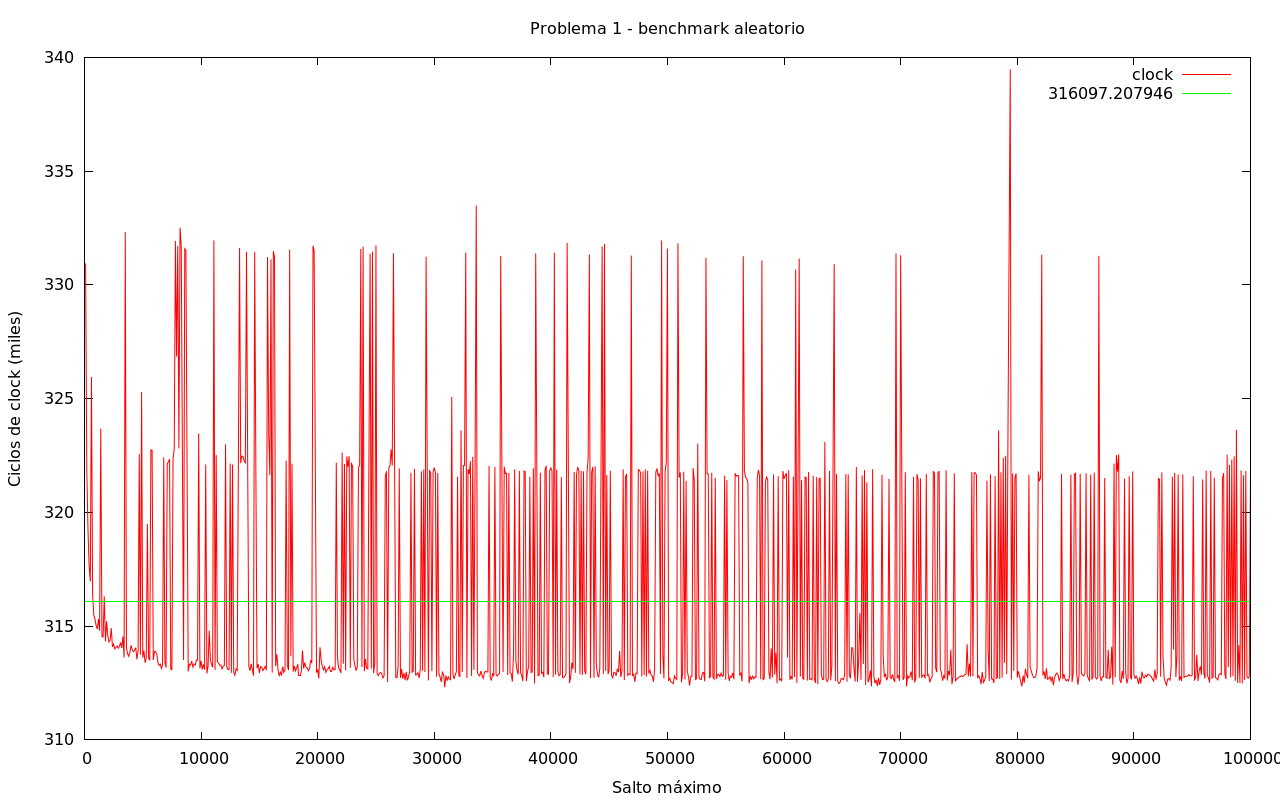
\includegraphics[scale=0.35]{imagenes/grafico-1-c.png}
  \end{center}
\end{figure}

